%%%%%%%%%%%%%%%%%%%%%%%%%%%%%%%%%%%%%%%%%%%%%%%%%%%%%%%%%%%%%%%%%%%%%%
% How to use writeLaTeX: 
%
% You edit the source code here on the left, and the preview on the
% right shows you the result within a few seconds.
%
% Bookmark this page and share the URL with your co-authors. They can
% edit at the same time!
%
% You can upload figures, bibliographies, custom classes and
% styles using the files menu.
%
%%%%%%%%%%%%%%%%%%%%%%%%%%%%%%%%%%%%%%%%%%%%%%%%%%%%%%%%%%%%%%%%%%%%%%

\documentclass[12pt]{article}


\usepackage{sbc-template}
\usepackage{graphicx, url}

\usepackage[brazil]{babel}   
\usepackage[utf8]{inputenc}  




%\renewcommand{\refname}{Referências}

\sloppy

\title{Um estudo preliminar sobre o uso de uma arquitetura deep learning para seleção de respostas no problema de recuperação de código-fonte}

% !!!! IMPORTANTE: O evento adota a política de double blind - deixe como anonimo para subtmeter!!!
% \author{Marcelo de Rezende Martins\inst{1}, Marco Aurélio Gerosa\inst{2}}


%\address{Instituto de Pesquisas Tecnológicas
%   (IPT)\\
%   São Paulo -- SP -- Brazil
% \nextinstitute
%   Northern Arizona University\\
%   Flagstaff, AZ, US
%   \email{rezende.martins@gmail.com, Marco.Gerosa@nau.edu}
% }

\begin{document} 

\maketitle

\begin{abstract}
  Code retrieval techniques aim to select a code snippet to solve a question given a set of possible solutions. This article presents a preliminary study about a new approach for code retrieval, applying an answer selection deep learning architecture. We present preliminary results of a bidirectional LSTM with convolutional network model adapted for code retrieval. After 20 runs on a evaluation dataset, our model could achieve a mean MRR of $0.60 \pm 0.02$ and a top-1 accuracy up to 51\%.
\end{abstract}
     
\begin{resumo} 
  Dado uma questão e um conjunto de trechos de código-fonte, recuperação de código-fonte ou \textit{code retrieval} busca encontrar o código que soluciona a dada questão. Este artigo apresenta um estudo preliminar sobre uma nova abordagem para o problema de recuperação de código-fonte, utilizando uma arquitetura deep learning de seleção de respostas. Apresentamos os resultados preliminares do modelo de redes neurais recorrentes bidirecionais (bi-LSTM) com redes neurais convolucionais (CNN) adaptado para o problema de recuperação de código-fonte. Após 20 execuções na amostra de teste, nosso modelo conseguiu atingir uma média MRR de $0,60 \pm 0,02$ e a medida top-1 o máximo de 51\%.
  % Fechar o resumo e abstract com uma sumarização dos resultados encontrados
\end{resumo}


\section{Introdução}

Segundo \cite{Allamanis-bimodal-source-code-natural-language:2015}, recuperação de código-fonte (\textit{code retrieval}) é um problema de recuperação de informação, onde dado uma questão ou uma descrição em linguagem natural e um conjunto de possíveis trechos de código-fonte, o objetivo é recuperar o trecho de código-fonte que solucione a questão ou seja mais relevante de acordo com a descrição. Já segundo \cite{lai-etal-2018-review}, dado uma questão e um conjunto de possíveis respostas, ambos em linguagem natural, seleção de respostas ou \textit{answer selection} busca identificar qual resposta consegue responder a pergunta corretamente. 

% motivação
O problema do \textit{code retrieval} busca associar um texto em linguagem natural a um código-fonte. Esta associação tem diversas aplicações como busca de código-fonte a partir de uma consulta em linguagem natural, documentação e geração de programas a partir de uma especificação, por exemplo \cite{Allamanis:2018:SML}. Em engenharia de software a associação entre código-fonte e texto em linguagem natural pode auxiliar na rastreabilidade de requisitos. Além disso, pode ajudar o desenvolvedor na geração de código-fonte. Um modelo pode gerar testes de unidade a partir de uma estória de usuário.

\cite{iyer-etal-2016-summarizing} em seu trabalho sobre \textit{code retrieval} propuseram um modelo deep learning formado por uma rede neural recorrente, mais especificamente o LSTM, com o mecanismo de atenção para solucionar o problema. Tanto LSTM quanto o mecanismo de atenção são comumente utilizados nos problemas de tradução e geração de texto \cite{bahdanau2014neural, rush-etal-2015-neural}. Para \cite{Allamanis:2018:SML}, software é uma forma de comunicação humana e tem propriedades estatísticas similares a corpora de linguagem natural. 

Este presente artigo busca apresentar os resultados preliminares de um estudo sobre o uso de arquitetura deep learning de \textit{answer selection} no problema do \textit{code retrieval}. Inicialmente, utilizaremos a arquitetura bi-LSTM com CNN proposta por \cite{tan-lstm-qa}. Além de propor uma nova arquitetura para este problema, avaliamos o modelo utilizando os dados de entrada da base StaQC, criada por \cite{Yao-staqc:2018}. Esta base de dados é composta de milhares de pares de perguntas e trechos de código-fonte do StackOverFlow. Para avaliar os dados, \cite{Yao-staqc:2018} utilizaram a arquitetura proposta por \cite{iyer-etal-2016-summarizing} e criaram um modelo composto por rede neural com o mecanismo de atenção. Esta arquitetura utilizada por \cite{iyer-etal-2016-summarizing} é comumente utilizada na geração de textos, que foi a proposta dele. 

 A nossa proposta inicial é apenas recuperar o trecho de código-fonte a partir de uma descrição, ou seja, o nosso foco é o problema do \textit{code retrieval}.



% \section{Trabalhos relacionados} \label{sec:trabrel}
% % Trouxe umas partes da intro para cá, mas precisa elaborar mais relatando outros trabalhos que abordam code retrieval, answer selection e deep learning

% Para \cite{Knuth:1984:LP}, 
% o código-fonte é uma forma de comunicação:

% \textit{"Let us change our traditional attitude to the construction of programs: Instead of imagining that our main task is to instruct a computer what to do, let us concentrate rather on explaining to human beings what we want a computer to do."}

% E \cite{Allamanis:2018:SML} apresenta a hipótese da naturalidade do código-fonte:

% \textit{"\textbf{The naturalness hypothesis}. Software is a form of human communication; software corpora have similar statistical properties to natural language corpora; and these properties can be exploited to build better software engineering tools."}

% Considerando o código-fonte uma forma de comunicação, assim elencado por \cite{Knuth:1984:LP} e reforçado por \cite{Allamanis:2018:SML} em sua hipótese, uma possível abordagem para o problema 
% do \textit{code retrieval}, é analisá-la sob a perspectiva do \textit{answer selection}. Porém, é necessário levar em consideração as peculiaridades do código-fonte ao abordar o problema sob esta perspectiva. 


\section{Método} \label{sec:metodo}

Conforme mencionado anteriormente, neste trabalho abordamos o problema do \textit{code retrieval} sob a perspectiva do \textit{answer selection}. Utilizamos 
a arquitetura proposta por \cite{tan-lstm-qa}, que utiliza a função de classificação \textit{pairwise} e uma arquitetura siamesa, de acordo com \cite{lai-etal-2018-review}. Para 
\cite{lai-etal-2018-review}, o problema de \textit{answer selection} pode ser analisado sob duas formas: forma de aprendizado e arquitetura.

\subsection{Forma de aprendizado}

O problema de \textit{answer selection} consiste em encontrar a resposta mais relevante dado uma questão. Ele pode ser abordado como uma problema de classificação, onde
o objetivo é classificar com uma pontuação melhor as respostas mais relevantes de acordo com a questão.

\cite{tan-lstm-qa} utilizaram o método \textit{pairwise}, no qual o objetivo da função é classificar as respostas corretas com uma pontuação maior que a das incorretas. Dado uma questão,
o método avalia o conjunto de repostas e aprende a classificar qual resposta é mais relevante para a questão. Por exemplo, o modelo proposto por \cite{tan-lstm-qa} e utilizado como referência neste artigo, os dados de entrada para o treinamento
são triplas $(q_{i}, c_{i}^{+}, c_{i}^{-})$, onde $q_{i}$ é uma questão, $c_{i}^{+}$ é uma resposta correta, $c_{i}^{-}$ é uma resposta incorreta. Seja a função de perda, \textit{hinge}, definida como:

\begin{equation}
L = max(0, m - h_{\theta}(q_{i}, c_{i}^{+}) + h_{\theta}(q_{i}, c_{i}^{-}))   
\end{equation}


Onde $m$ é a margem. Se $h_{\theta}(q_{i}, c_{i}^{+}) - h_{\theta}(q_{i}, c_{i}^{-}) < m$ então $L$ é positivo. Quando esta condição é satisfeita, a implicação é que o sistema classifica a resposta correta abaixo da resposta incorreta, ou a questão correta pontua um pouco acima da resposta incorreta. Por outro lado, se a resposta correta tem uma pontuação maior que a incorreta por uma margem acima ou igual a $m$ (i.e., $h_{\theta}(q_{i}, c_{i}^{+}) - h_{\theta}(q_{i}, c_{i}^{-}) \geq m$, a função de perda é igual a zero. Em resumo, a função de perda incentiva a reposta correta a ter uma pontuação maior que a incorreta por uma certa margem \cite{lai-etal-2018-review}.

\cite{tan-lstm-qa} propuseram o uso da função de similaridade \textit{cosine}. Esta função de similaridade é comumente utilizada em problemas de \textit{answer selection} \cite{feng-answer-selection-2015}. 

\subsection{Arquitetura}

\cite{tan-lstm-qa} propuseram uma arquitetura que utiliza uma rede neural recorrente bidirecional, mais especificamente uma rede LSTM (biLSTM) \cite{hochreiter-Schmidhuber-lstm-1997} e uma camada pooling para construir a representação dos vetores de entrada. Ao final, o modelo utiliza a função de similaridade \textit{cosine} para calcular a distância
entre as representações. 

A arquitetura de referência que iremos utilizar acrescenta uma estrutura de rede convolucional na saída da rede bi-LSTM. Os vetores de saída da rede bi-LSTM tornam-se vetores de entrada na na estrutura CNN. O CNN auxilia na síntese da representação dos vetores. A imagem ilustrativa da arquitetura pode ser visualizada na Figura~\ref{fig:arquitetura-bi-lstm}.


\begin{figure}[h]
    \centering
    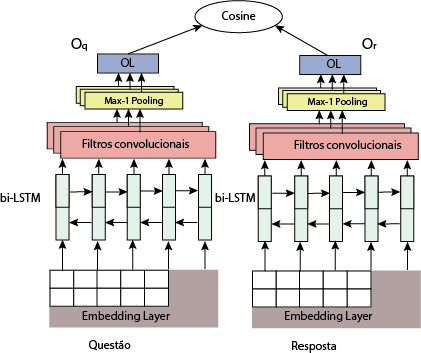
\includegraphics[width=0.60\textwidth]{figures/ArquiteturaBiLSTM.png}
    \caption{Figura da arquitetura proposta para o problema do \textit{code retrieval}. Figura adaptada do \cite{tan-lstm-qa}}
    \label{fig:arquitetura-bi-lstm}
\end{figure}

% Dar todos os detalhes de configuração de modo que qualquer pessoa possa replicar o seu estudo e obter os mesmo rsultados



% Criar uma secao para faalr do seu data set

\section{Experimento}\label{sec:experimento}

Para avaliar a arquitetura proposta por \cite{tan-lstm-qa} composta por uma rede bi-LSTM com CNN no problema do \textit{code retrieval}, utilizamos os dados disponibilizados por \cite{Yao-staqc:2018}. Em seu trabalho \cite{Yao-staqc:2018} coletaram mais de \textbf{147 mil} pares de perguntas e trechos de código-fonte em Python e aproximadamente \textbf{119 mil} pares de perguntas e trechos de código-fonte em SQL. 

\begin{table}[h]
\centering
\begin{tabular}{ |p{3cm}|r|r|r|r|  }
\hline
&\multicolumn{2}{|c|}{\textbf{Questão}} & \multicolumn{2}{|c|}{\textbf{Código-Fonte}} \\
\hline
& \textbf{Tamanho} & \textbf{\# de palavras} & \textbf{Tamanho} & \textbf{\# de palavras}\\
 \hline
 \textbf{Média} & $51,60$ & $8,9$ & $326$ & $48,84$\\
 \hline
 \textbf{Desvio Padrão} & $18,57$ & $3,64$ & $477$ & $65,79$\\
 \hline
 \textbf{Mínimo} & $13$ & $2$ & $4$ & $0$\\
 \hline
 \textbf{25\%} & $38$ & $6$ & $95$ & $16$\\
 \hline
 \textbf{50\%} & $49$ & $8$ & $192$ & $31$\\
 \hline
 \textbf{75\%} & $62$ & $11$ & $380$ & $58$\\
 \hline
 \textbf{Máximo} & $150$ & $32$ & $17200$ & $3170$\\
 \hline
\end{tabular}
\caption{Estatísticas da amostra de 62252 pares $(q_{i}, c_{i}^{+})$ em Python}
\label{table:divisao-amostras}
\end{table}



Inicialmente, utilizaremos uma amostra de 62252 pares $(q_{i}, c_{i}^{+})$ em Python. Onde $q_{i}$ é o título de uma questão no site StackOverFlow\footnote{Site: https://www.stackoverflow.com/} e $c_{i}^{+}$ corresponde a um trecho de código-fonte apontado como solução para a questão $q_{i}$. Destes 62252 pares, excluímos 2169 pares que foram anotados manualmente. Estes 2169 pares $(q_{i}, c_{i}^{+})$ anotados manualmente serão divididos em duas amostras: \emph{DEV} e \emph{EVAL}.


\begin{table}[h]
\centering
\begin{tabular}{ |p{3cm}|p{3cm}|  }
 \hline
 \textbf{Amostras} & \textbf{Quantidade de $(q_{i}, c_{i}^{+})$}\\
 \hline
 Treinamento & $60083$\\
 \hline
 DEV & $1085$ \\
 \hline
 EVAL & $1084$\\
 \hline
 \textbf{Total} & $62252$\\
 \hline
\end{tabular}
\caption{Divisão das amostras conforme os critérios adotados por \cite{iyer-etal-2016-summarizing}}
\label{table:divisao-amostras}
\end{table}

% Rever todo o texto e não usar o futuro para descrever o método. Usar o passado ou presente.
Conforme a tabela~\ref{table:divisao-amostras}, utilizaremos 60083 pares $(q_{i}, c_{i}^{+})$ para treinamento. Para obter o modelo, adotamos o mesmo procedimento proposto por \cite{iyer-etal-2016-summarizing}. No caso, o modelo será treinado, inicialmente, durante 80 épocas. Caso o \textit{learning rate} fique abaixo de 0,001, o treinamento é interrompido. Ao final de cada época, o modelo é avaliado na amostra \emph{DEV}. 


A avaliação na amostra \emph{DEV} consiste em avaliar a qualidade do modelo calculando o \textit{Mean Reciprocal Rank} (MRR). Esta avaliação é feita da seguinte forma:
 Para cada par $(q_{i}, c_{i}^{+})$ na amostra \emph{DEV}, selecionaremos outros 49 distratores $c^{'}$ da amostra de treinamento, onde $c^{'} \neq c_{i}^{+}$. Estes 50 pares $(c_{i}, q_{i})$ serão classificados de acordo com a função $h_{\theta}$ de similaridade. Posteriormente, o MRR de cada questão $q_{i}$ é calculado. Ao final, calculamos a média do valor do MRR. O modelo de treinamento que obter a maior média MRR na amostra \emph{DEV} será escolhido. 
 
 
 
 Após o término do treinamento e com o modelo com a maior média MRR na amostra \emph{DEV} escolhido, a avaliação final é feita. Durante a avaliação final, a qualidade do modelo é avaliado na amostra \emph{EVAL}. O procedimento é o mesmo adotado para avaliar o modelo na amostra \emph{DEV}.


\subsection{Configuração}

Os dados foram representados como sequência de tokens. Utilizamos uma representação distribuída word2vec \cite{mikolov-word2vec-2013}. Diferente do \textit{answer selection} proposto por \cite{tan-lstm-qa} no qual ele cria apenas uma representação distribuída para a amostra inteira, nós geramos a representação distribuída para as questões e outra para os trechos do código-fonte.

Quanto ao código-fonte, foi feito um pré-processamento. Utilizamos a função disponibilizada por \cite{Yao-staqc:2018} que substitui literais numéricos e texto (\textit{string}) por NUMBER e STRING. Os comentários são removidos e o nome das variáveis são substituídas por VAR.

Os parâmetros de execução foram os mesmos utilizados por \cite{tan-lstm-qa}. Com exceção dos filtros na camada CNN, que reduzimos para o valor 100. O valor utilizado por \cite{tan-lstm-qa} de 1000, aumentou a capacidade do modelo, causando o \textit{overfitting}.




\section{Resultados preliminares}\label{sec:resultados-preliminares}

Os resultados do experimento podem ser visualizados na tabela~\ref{table:resultados-preliminares}. Os resultados correspondem a média do MRR após 20 rodadas de execução utilizando o melhor modelo obtido a partir do treinamento. E o modelo foi avaliado na amostra \emph{EVAL}. 

Nestes resultados preliminares, comparamos o modelo bi-LSTM com CNN com outros dois modelos. O modelo \emph{Embedding}, mais simples, é composto apenas por uma camada com a representação distribuída das questões e trechos de código-fonte. A saída é uma camada de \textit{maxpool} e ao final a similaridade é calculada através da função \textit{cosine}. 

O modelo \emph{CNN} é uma rede neural convolucional com uma camada \textit{hidden} de entrada \emph{HL}. Esta camada \textit{hidden}  é definida como $z = tanh(Wx +B)$. Onde $W$ é a matriz de pesos; $B$ é o vetor \textit{bias}; $x$ é o vetor de entrada; $z$ é o resultado da função de ativação $tanh$.  Este modelo utiliza também o \textit{maxpool} e a mesma função de similaridade.

Imagens ilustrativas das arquiteturas dos modelos \emph{Embedding} e \emph{CNN} podem ser visualizadas nas Figura~\ref{fig:arquitetura-embedding} e Figura~\ref{fig:arquitetura-cnn}, respectivamente.

\begin{figure}[h]
    \centering
    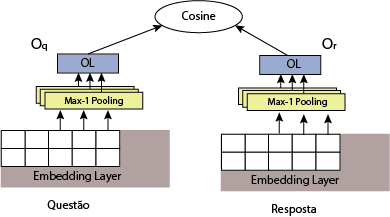
\includegraphics[width=0.60\textwidth]{figures/ArquiteturaEmbedding.png}
    \caption{Figura da arquitetura \emph{Embedding}. Figura adaptada do \cite{tan-lstm-qa}}
    \label{fig:arquitetura-embedding}
\end{figure}

\begin{figure}[h]
    \centering
    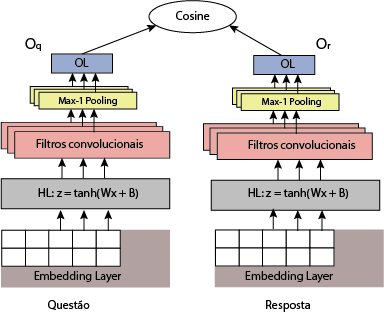
\includegraphics[width=0.60\textwidth]{figures/ArquiteturaCNN.png}
    \caption{Figura da arquitetura \emph{CNN}. Figura adaptada do \cite{tan-lstm-qa}}
    \label{fig:arquitetura-cnn}
\end{figure}

A implementação dos modelos foi feito utilizando a biblioteca Keras. O código de implementação e o resultados preliminares estão disponíveis no repositório Git \url{https://github.com/ANONYMOUS}. Além disso, os dados pré-processados podem ser visualizados no repositório \url{https://github.com/ANONYMOUS}.

De acordo com a tabela~\ref{table:resultados-preliminares}, \textbf{bi-LSTM-CNN} obteve o melhor desempenho. Porém, CNN obteve um resultado muito próximo e o tempo de treinamento é muito menor. O tempo total de treinamento da rede bi-LSTM com CNN levou em torno de 48 minutos, utilizando uma GPU Tesla K80. Enquanto a arquitetura CNN levou em torno de 6s. 

Em todos os modelos, utilizamos uma camada de \textit{maxpool} e a função de similaridade \textit{cosine}. Utilizamos o valor de margem $0,009$ para a função de perda \textit{hinge}, valor proposto por \cite{feng-answer-selection-2015}.


\begin{table}[h]
\centering
\begin{tabular}{ |p{3cm}|p{3cm}|  }
 \hline
 \textbf{Modelos} & \textbf{MRR}\\
 \hline
 Embedding & $0,52 \pm 0,01$\\
 \hline
 CNN & $0,58 \pm 0,01 $ \\
 \hline
 \textbf{bi-LSTM-CNN} & $\textbf{0,60} \pm \textbf{0,02}$\\
 \hline
\end{tabular}
\caption{Resultados preliminares dos modelos QA de \cite{tan-lstm-qa} no problema de \textit{code retrieval}}
\label{table:resultados-preliminares}
\end{table}

\subsection{Ameaças à validade}

Os dados utilizados no treinamento para obter o modelo final foram coletados automaticamente por \cite{Yao-staqc:2018}. \cite{Yao-staqc:2018} criaram um modelo composto por uma rede neural recorrente para obter os pares de questões e trechos de código-fonte automaticamente. E para treinar este modelo, foi utilizado os dados anotados manualmente. Estes dados anotados manualmente (amostras \emph{DEV} e \emph{EVAL}) são os mesmos utilizados na avaliação do nosso modelo. 

Para minimizar o viés, utilizamos o mesmo procedimento de avaliação proposto por \cite{iyer-etal-2016-summarizing}. Para cada par de $(q_{i}, c_{i}^{+})$, selecionamos aleatoriamente 49 distratores $c^{'}$ da amostra de treinamento, onde $c^{'} \neq c_{i}$. 

\section{Conclusões}\label{sec:conclusao}

Neste trabalho, propusemos uma abordagem diferente para o problema do \textit{code retrieval}. Nosso intuito foi abordar o problema do \textit{code retrieval} sob a perspectiva do problema \textit{answer selection}, já conhecido em NLP. E dado o bom desempenho dos modelos deep learning no contexto do \textit{answer selection}, utilizamos o modelo proposto por \cite{tan-lstm-qa}.

Conforme a Seção~\ref{sec:resultados-preliminares}, o modelo proposto por \cite{tan-lstm-qa} apresentou um bom desempenho. O valor médio de MRR de $0,60 \pm 0,02$ é um valor expressivo. Este resultado preliminar serve como um indicativo para aprimorarmos o modelo para o problema do \textit{code retrieval}. \cite{Yao-staqc:2018} obtiveram uma média MRR de $0,57 \pm 0,02$ e \cite{iyer-etal-2016-summarizing} obtiveram $0,44 \pm 0,01$, porém numa amostra de pares de questões e códigos-fontes em SQL disponibilizada por \cite{iyer-etal-2016-summarizing}. O próximo passo é avaliarmos a nossa arquitetura utilizando os mesmos dados e procedimentos proposto por \cite{Yao-staqc:2018}. 

Além disso, como citado por \cite{lai-etal-2018-review}, trabalhos futuros podem aplicar o modelo BiMPM (\textit{Bilateral Multi-Perspective Matching for Natural Language Sentences}) proposto por \cite{wang-BiMPM-2017}, que apresentou um bom desempenho no problema de \textit{answer selection}.

Uma frente ainda a ser explorada no problema do \textit{code retrieval} é a disponibilização de dados para avaliação dos modelos. A área de reconhecimento de imagem tem o \textit{ImageNet} \cite{imagenet_cvpr09} um vasto banco de dados com mais de 14 milhões de imagens anotados manualmente. A área de inferência em linguagem natural para determinar se uma hipótese é verdadeira, falsa ou neutra contém mais de 570 mil sentenças em inglês anotadas manualmente \cite{snli:emnlp2015}. 

O próprio problema de \textit{answer selection} utiliza Trec-QA \cite{wang-etal-2007-jeopardy} e InsuranceQA \cite{feng-answer-selection-2015}. O trabalho de \cite{Yao-staqc:2018} anotou 4884 pares de questões e trechos de código-fonte manualmente. Isto é um passo importante e conforme mais dados curados e organizados forem disponibilizados, mais a área de \textit{machine learning} aplicado a código-fonte e engenharia de software tende a ganhar.





\bibliographystyle{sbc}
\bibliography{sbc-template}


\end{document}